% Options for packages loaded elsewhere
\PassOptionsToPackage{unicode}{hyperref}
\PassOptionsToPackage{hyphens}{url}
\PassOptionsToPackage{dvipsnames,svgnames,x11names}{xcolor}
%
\documentclass[
  11pt,
]{article}

\usepackage{amsmath,amssymb}
\usepackage{iftex}
\ifPDFTeX
  \usepackage[T1]{fontenc}
  \usepackage[utf8]{inputenc}
  \usepackage{textcomp} % provide euro and other symbols
\else % if luatex or xetex
  \usepackage{unicode-math}
  \defaultfontfeatures{Scale=MatchLowercase}
  \defaultfontfeatures[\rmfamily]{Ligatures=TeX,Scale=1}
\fi
\usepackage{lmodern}
\ifPDFTeX\else  
    % xetex/luatex font selection
\fi
% Use upquote if available, for straight quotes in verbatim environments
\IfFileExists{upquote.sty}{\usepackage{upquote}}{}
\IfFileExists{microtype.sty}{% use microtype if available
  \usepackage[]{microtype}
  \UseMicrotypeSet[protrusion]{basicmath} % disable protrusion for tt fonts
}{}
\makeatletter
\@ifundefined{KOMAClassName}{% if non-KOMA class
  \IfFileExists{parskip.sty}{%
    \usepackage{parskip}
  }{% else
    \setlength{\parindent}{0pt}
    \setlength{\parskip}{6pt plus 2pt minus 1pt}}
}{% if KOMA class
  \KOMAoptions{parskip=half}}
\makeatother
\usepackage{xcolor}
\usepackage[margin=1in]{geometry}
\setlength{\emergencystretch}{3em} % prevent overfull lines
\setcounter{secnumdepth}{5}
% Make \paragraph and \subparagraph free-standing
\ifx\paragraph\undefined\else
  \let\oldparagraph\paragraph
  \renewcommand{\paragraph}[1]{\oldparagraph{#1}\mbox{}}
\fi
\ifx\subparagraph\undefined\else
  \let\oldsubparagraph\subparagraph
  \renewcommand{\subparagraph}[1]{\oldsubparagraph{#1}\mbox{}}
\fi


\providecommand{\tightlist}{%
  \setlength{\itemsep}{0pt}\setlength{\parskip}{0pt}}\usepackage{longtable,booktabs,array}
\usepackage{calc} % for calculating minipage widths
% Correct order of tables after \paragraph or \subparagraph
\usepackage{etoolbox}
\makeatletter
\patchcmd\longtable{\par}{\if@noskipsec\mbox{}\fi\par}{}{}
\makeatother
% Allow footnotes in longtable head/foot
\IfFileExists{footnotehyper.sty}{\usepackage{footnotehyper}}{\usepackage{footnote}}
\makesavenoteenv{longtable}
\usepackage{graphicx}
\makeatletter
\def\maxwidth{\ifdim\Gin@nat@width>\linewidth\linewidth\else\Gin@nat@width\fi}
\def\maxheight{\ifdim\Gin@nat@height>\textheight\textheight\else\Gin@nat@height\fi}
\makeatother
% Scale images if necessary, so that they will not overflow the page
% margins by default, and it is still possible to overwrite the defaults
% using explicit options in \includegraphics[width, height, ...]{}
\setkeys{Gin}{width=\maxwidth,height=\maxheight,keepaspectratio}
% Set default figure placement to htbp
\makeatletter
\def\fps@figure{htbp}
\makeatother
\newlength{\cslhangindent}
\setlength{\cslhangindent}{1.5em}
\newlength{\csllabelwidth}
\setlength{\csllabelwidth}{3em}
\newlength{\cslentryspacingunit} % times entry-spacing
\setlength{\cslentryspacingunit}{\parskip}
\newenvironment{CSLReferences}[2] % #1 hanging-ident, #2 entry spacing
 {% don't indent paragraphs
  \setlength{\parindent}{0pt}
  % turn on hanging indent if param 1 is 1
  \ifodd #1
  \let\oldpar\par
  \def\par{\hangindent=\cslhangindent\oldpar}
  \fi
  % set entry spacing
  \setlength{\parskip}{#2\cslentryspacingunit}
 }%
 {}
\usepackage{calc}
\newcommand{\CSLBlock}[1]{#1\hfill\break}
\newcommand{\CSLLeftMargin}[1]{\parbox[t]{\csllabelwidth}{#1}}
\newcommand{\CSLRightInline}[1]{\parbox[t]{\linewidth - \csllabelwidth}{#1}\break}
\newcommand{\CSLIndent}[1]{\hspace{\cslhangindent}#1}

\makeatletter
\makeatother
\makeatletter
\makeatother
\makeatletter
\@ifpackageloaded{caption}{}{\usepackage{caption}}
\AtBeginDocument{%
\ifdefined\contentsname
  \renewcommand*\contentsname{Table of contents}
\else
  \newcommand\contentsname{Table of contents}
\fi
\ifdefined\listfigurename
  \renewcommand*\listfigurename{List of Figures}
\else
  \newcommand\listfigurename{List of Figures}
\fi
\ifdefined\listtablename
  \renewcommand*\listtablename{List of Tables}
\else
  \newcommand\listtablename{List of Tables}
\fi
\ifdefined\figurename
  \renewcommand*\figurename{Figure}
\else
  \newcommand\figurename{Figure}
\fi
\ifdefined\tablename
  \renewcommand*\tablename{Table}
\else
  \newcommand\tablename{Table}
\fi
}
\@ifpackageloaded{float}{}{\usepackage{float}}
\floatstyle{ruled}
\@ifundefined{c@chapter}{\newfloat{codelisting}{h}{lop}}{\newfloat{codelisting}{h}{lop}[chapter]}
\floatname{codelisting}{Listing}
\newcommand*\listoflistings{\listof{codelisting}{List of Listings}}
\makeatother
\makeatletter
\@ifpackageloaded{caption}{}{\usepackage{caption}}
\@ifpackageloaded{subcaption}{}{\usepackage{subcaption}}
\makeatother
\makeatletter
\@ifpackageloaded{tcolorbox}{}{\usepackage[skins,breakable]{tcolorbox}}
\makeatother
\makeatletter
\@ifundefined{shadecolor}{\definecolor{shadecolor}{rgb}{.97, .97, .97}}
\makeatother
\makeatletter
\makeatother
\makeatletter
\makeatother
\ifLuaTeX
  \usepackage{selnolig}  % disable illegal ligatures
\fi
\IfFileExists{bookmark.sty}{\usepackage{bookmark}}{\usepackage{hyperref}}
\IfFileExists{xurl.sty}{\usepackage{xurl}}{} % add URL line breaks if available
\urlstyle{same} % disable monospaced font for URLs
\hypersetup{
  pdftitle={Final Project Report},
  pdfauthor={Catherine Jackson (ccj3)},
  colorlinks=true,
  linkcolor={blue},
  filecolor={Maroon},
  citecolor={Blue},
  urlcolor={Blue},
  pdfcreator={LaTeX via pandoc}}

\title{Final Project Report}
\author{Catherine Jackson (ccj3)}
\date{Tue., Apr.~30}

\begin{document}
\maketitle
\ifdefined\Shaded\renewenvironment{Shaded}{\begin{tcolorbox}[interior hidden, sharp corners, borderline west={3pt}{0pt}{shadecolor}, enhanced, frame hidden, breakable, boxrule=0pt]}{\end{tcolorbox}}\fi

\hypertarget{introduction}{%
\section{Introduction}\label{introduction}}

\hypertarget{storm-surge-variability-and-literature-review}{%
\subsection{Storm Surge Variability and Literature
Review}\label{storm-surge-variability-and-literature-review}}

Hurricanes represent an ever-present threat to US coastlines, and these
events have incredible potential to damage infrastructure and threaten
lives. In fast, (\textbf{ncei2024?}) found that, when analyzing data
from 1980 to 2024, damages from tropical cyclones and severe storms
account for 51.8\% and 17.3\% of climate disaster-related costs. These
severe storms and their associated surge events must be better
understood in order to protect communities from their damages.

However, both the frequency and characteristics of these storms and
their associated surges is made more complex due to spatial
dependencies. (\textbf{Needham2012?}) sought to create a storm surge
database based on historical activity. They argue that this database can
be used by communities to better protect themselves based on historical
data. They found that the Central and Western Gulf Coast is particularly
vulnerable to hurricanes, both in terms of increased frequency and
magnitude, as well as storm surge. Comparatively, the East Coast
experienced less frequenct and smaller events. Furthermore,
(\textbf{Xu2010?}) hoped to better understand how the incorporation of
multi-scale simulations, but their results also demonstrated that
differences in coastal tophography and bathymetry led to large
variations in storm surge events. (\textbf{islam2021new?}) found similar
results. After including information about translational speed and
coastal geometry, the predictions from their surge index became
significantly more accurate. In this way, (\textbf{Needham2012?})
demonstrates that there are significant variations along the US
coastline based on hurricane magnitude and frequency, and the associated
storm surge, due to important climate variations. In addition,
(\textbf{Xu2010?}) and (\textbf{islam2021new?}) demonstrated that
including information about cosatal geometries and bathymetries is
important to accurately modeling and predicting surge.

The image below, from (\textbf{Needham2012?}), visually shows the
differences in storm surge across the Southern US coastline based on
historical information and data.

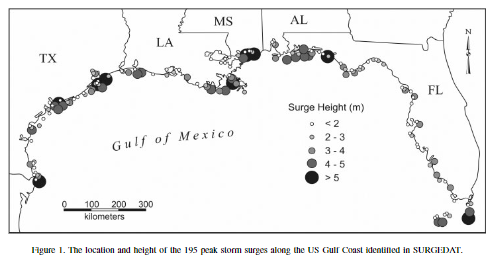
\includegraphics{/Needham2012Figure1.PNG}

These papers all demonstrate that physical differences in the coast as
well as climate differences in the storms themselves mean that surge
behavior is incredibly spatial. To accurately protect communities and
analyze risk, the spatial trends must be understood and regional data
must be included.

\hypertarget{problem-statement}{%
\subsection{Problem Statement}\label{problem-statement}}

In the original risk analysis code, a representative storm surge is
randomly generated. This storm surge is represented with a GEV
distribution defined by three parameters, each being generated from its
own distribution. Most importantly, though, this function was used to
apply regardless of the site of interest. The same function was used at
many different points across the coastline. As discussed above, however,
it is important to include spatial variability given that severe storms
and associated surges are highly dependent on the location along the
coast and nearby geometry and bathymetry.

\textbf{The problem that must be addressed, then, is a methodology by
which spatial information can be incorporated into the surge function
such that the surge is more accurate given the physical characteristics
and location of the site.}

It is important to address this lack of spatial specificity in the
current storm surge generation, within the context of climate risk
analysis, as, even if the climate risk assessment methodology is
appropriate and efficient, it is dependent on the quality of incoming
data. For example, a project could have a statistically sound
methodology of determining whether to raise a house given certain flood
risks, but if the storm surge distribution used is incorrectly low, the
model would incorrectly underestimate the true risk. Improving data
inputs improves the decisions produced by this risk analysis tool.

For these reasons, the surge distribution should be as accurate as
possible for the specific site of interest. The best methodology to do
so is to adjust this distribution towards the observational data from
the nearest gage.

\hypertarget{selected-feature}{%
\subsection{Selected Feature}\label{selected-feature}}

To address the spatial trends demonstrated in severe storms and
associated storm surge, the surge distribution used in risk analysis
must be specific to the site of interest. Therefore, the new addition to
the decision-support tool must shift the distribution such that it
better represents observed data at the nearest gage.

Describe the feature you have selected to add to the existing
decision-support tool. Discuss how this feature relates to the problem
statement and its potential to improve climate risk assessment.

\hypertarget{methodology}{%
\section{Methodology}\label{methodology}}

\hypertarget{implementation}{%
\subsection{Implementation}\label{implementation}}

You should make your modifications in either the \texttt{HouseElevation}
or \texttt{ParkingGarage} module. Detail the steps taken to implement
the selected feature and integrate it into the decision-support tool.
Include code snippets and explanations where necessary to clarify the
implementation process.

\hypertarget{validation}{%
\subsection{Validation}\label{validation}}

As we have seen in labs, mistakes are inevitable and can lead to
misleading results. To minimize the risk of errors making their way into
final results, it is essential to validate the implemented feature.
Describe the validation techniques used to ensure the accuracy and
reliability of your implemented feature. Discuss any challenges faced
during the validation process and how they were addressed.

\hypertarget{results}{%
\section{Results}\label{results}}

Present the results obtained from the enhanced decision-support tool.
Use tables, figures, and visualizations to clearly communicate the
outcomes. Provide sufficient detail to demonstrate how the implemented
feature addresses the problem statement. Use the
\texttt{\#\textbar{}\ output:\ false} and/or
\texttt{\#\textbar{}\ echo:\ false} tags to hide code output and code
cells in the final report except where showing the output (e.g.g, a
plot) or the code (e.g., how you are sampling SOWs) adds value to the
discussion. You may have multiple subsections of results, which you can
create using \texttt{\#\#}.

\hypertarget{conclusions}{%
\section{Conclusions}\label{conclusions}}

\hypertarget{discussion}{%
\subsection{Discussion}\label{discussion}}

Analyze the implications of your results for climate risk management.
Consider the context of the class themes and discuss how your findings
contribute to the understanding of climate risk assessment. Identify any
limitations of your approach and suggest potential improvements for
future work.

\hypertarget{conclusions-1}{%
\subsection{Conclusions}\label{conclusions-1}}

Summarize the key findings of your project and reiterate the
significance of your implemented feature in addressing the problem
statement. Discuss the broader implications of your work for climate
risk management and the potential for further research in this area.

\hypertarget{references}{%
\section{References}\label{references}}

\hypertarget{refs}{}
\begin{CSLReferences}{0}{0}
\end{CSLReferences}



\end{document}
